As a small, final example of an experimental determination of the Wigner function of quatnum states, I present the paper of Hofheinz et. al., 2009 \cite{Hofheinz}.

This architecture is different still than the optical platforms already discussed. It involves the use of superconducting circuits. But, the implementation follows the same math, so the results should be the same (excluding environmental differences between the two types of schemes). In not so many words, (because there is not room for many more), microwave pulses are applied to the qubit (see figure \ref{HofheinzSetUp}) to excite the qubit into an arbitrary superposition of $\ket{0}$ and $\ket{1}$. Initially, the qubit transition frequency is detuned (off-resonance) from the resonator frequency. This deters unwanted, spontaneous energy transfer from the qubit to the resonator. Once the state has been prepared in the qubit, the qubit is brought on resonance with the resonator and the exchange of a photon from the qubit to the resonator takes place. By repeatedly doing this and keeping track of the phase of old photons, one can generate arbitrary Fock states in the resonator. Then, the resonator can be probed and analyzed over many instantiations of the state of interest. This allows full tomography to be conducted on the state and the Wigner function to be determined. The results of their measurements are shown in figure \ref{HofheinzResults}.	

\begin{figure}%
\begin{center}
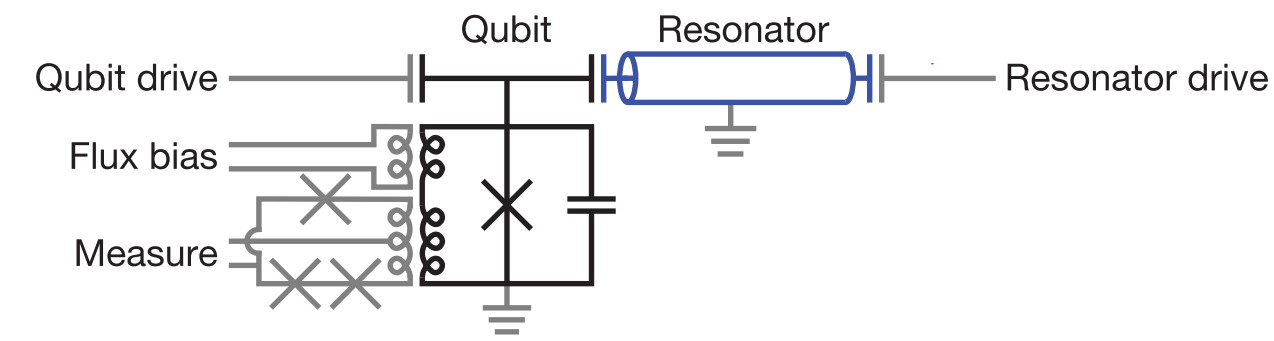
\includegraphics[width=300px,height=80px]{Figures/HofheinzSetUp.png}%
\caption{Circuit schematic of the superconducting circuit used in the Hofheinz et. al. paper of 2009.}%
\label{HofheinzSetUp}%
\end{center}
\end{figure}


\begin{figure}%
\begin{center}	
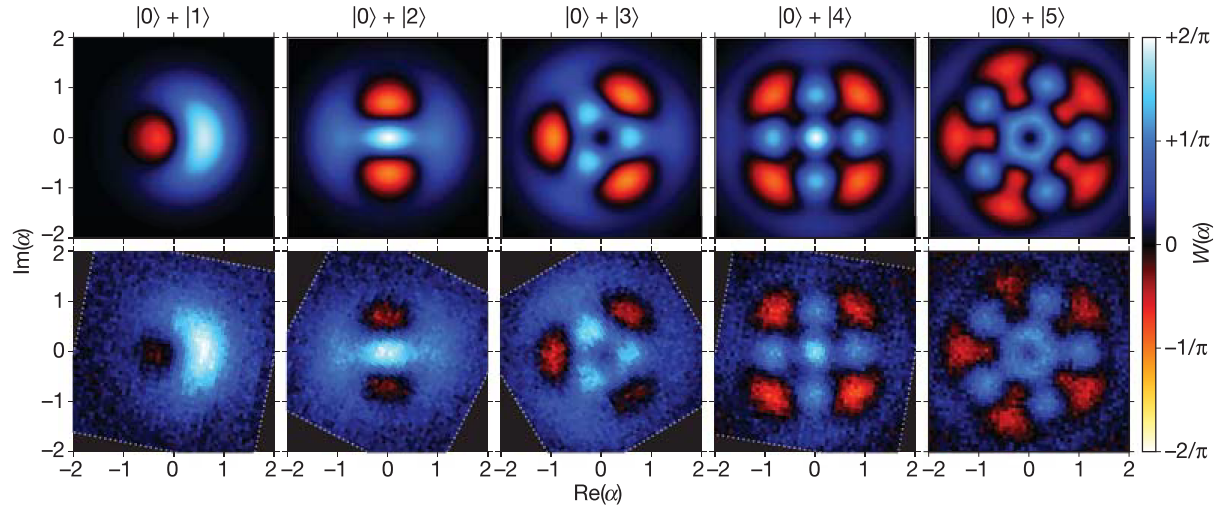
\includegraphics[width=300px,height=125px]{Figures/HofheinzResults.png}%
\caption{Results reported from the 2009 Hofheinz paper.}%
\label{HofheinzResults}%
\end{center}
\end{figure}
